\chapter{Introduction}
\label{chapter:1}

Social networks, or social media, can be defined as platforms that allow
individuals to connect to others, share personal information, and
provide content~\cite{boyd2007}. The information that flows in these
networks is not always public, but usually takes place by means of
private infrastructure that belongs to service providers.

In the context of computer security, privacy can be defined as someone's
capacity of controlling which information related to them can be consumed and
stored, and with whom it can be shared~\cite{stallings2010}. In addition to
guaranteeing their users' privacy, social networks must ensure the
confidentiality of the information they host, i.e. making sure that users'
private information is not exposed to unauthorized individuals.

It can be argued that a central provider having all the control over the
flow of private information would put user privacy in jeopardy,
for a few reasons. First, the central provider is a single point of
failure, and a security breach in its infrastructure exposes every user
of the service. Second, users are left with no option other than blindly
trusting the service provider to not misuse their personal information.
In the case of a commercial entity, that implies trusting the company
\textit{but also any other company that may acquire it in the future} to
not secretly violate its publicly available privacy policy, and to not
revise the privacy policy itself to include new terms that are not
favorable to its users.

\begin{figure}[!htbp]
	\centering
		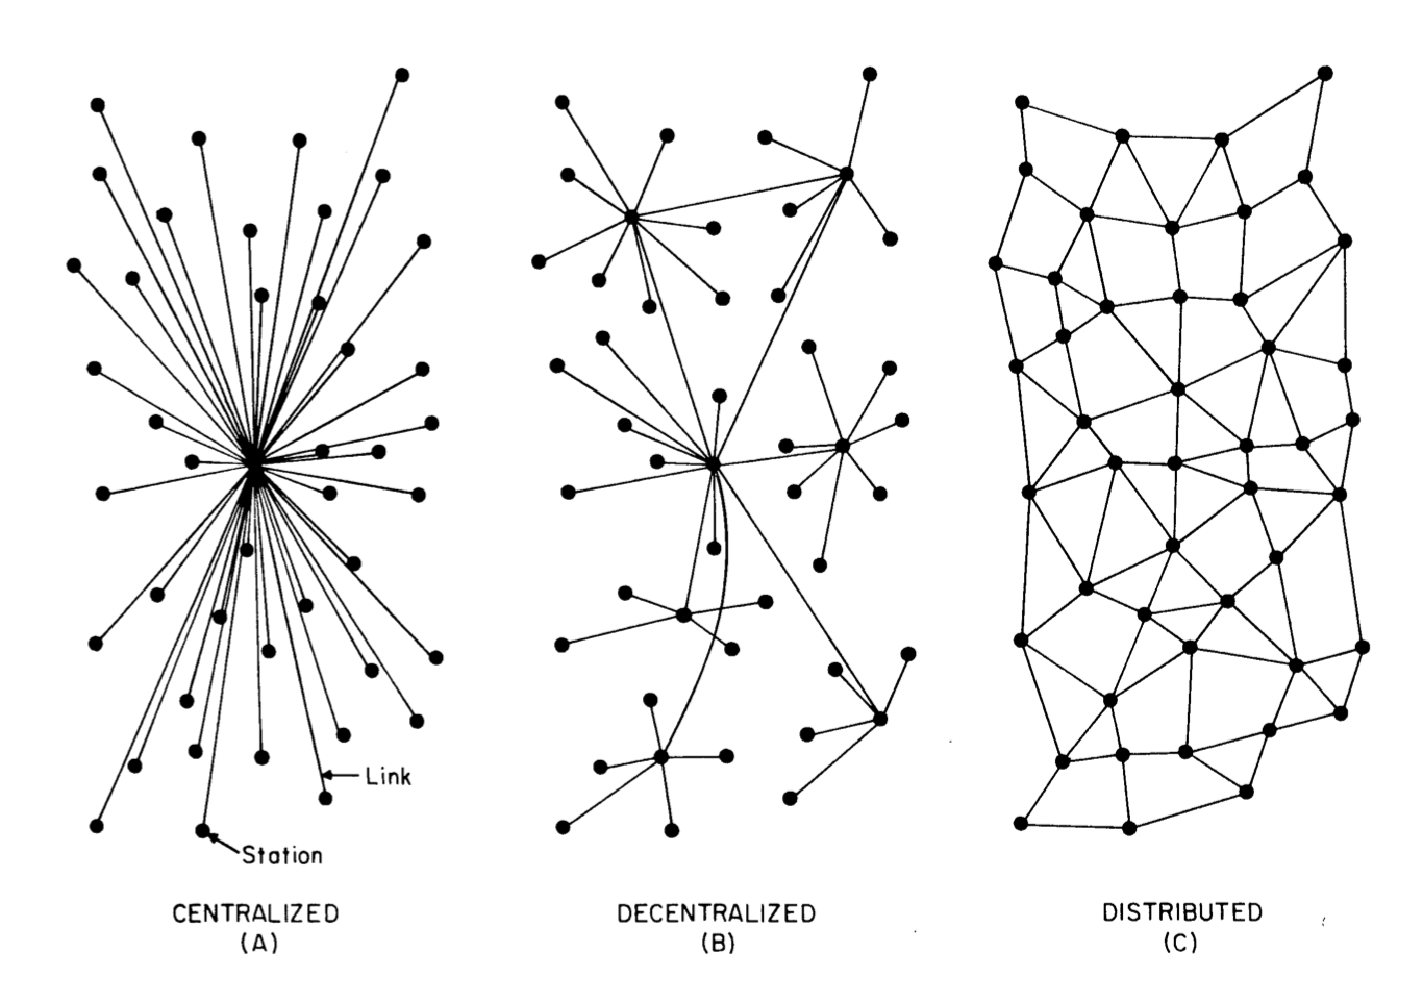
\includegraphics[keepaspectratio=true,scale=0.35]{figures/org_redes.eps}
	\caption{Conceptual models for communication networks (Source [1]).}
	\label{fig:org_redes}
\end{figure}

The concept of decentralized networks is an alternative to the centralization
of private data flow. Decentralization is even one of the original
characteristics of the Internet, and a common organization pattern in
communication networks. Communication networks can be centralized or
distributed~\cite{baran1964}. Centralized networks rely on a central node to
mediate communication between all the other nodes.  Decentralized networks have
multiple mediating nodes, while, in fully distributed networks, nodes can
communicate directly in any pattern that is possible and/or necessary. As
illustrated by Baran~\cite{baran1964} in Figure \ref{fig:org_redes}.

Centralized social networks, even if provided by a decentralized
infrastructure with the goal to improve performance and efficiency,
conceptually still follow a centralized network model. The central node
represents the service provider while the rest represents the millions
of users. Adopting a decentralized model means dividing users among
connected, intermediary providers that offer the same service,
guaranteeing interoperability, so that a user that is served by provider
``A'' can still interact with a user that is served by provider ``B''.

A set of interconnected servers that seamlessly provide a service is defined by
some authors as a federated network \cite{fednetworks}, which is similar to the
definition of decentralized networks shown in~\cite{baran1964}, but that is also
defined as a set of interoperable implementations that follow a client-server
model~\cite{barocas2012}.  This definition is important because it generalizes
the concept of federation to other types of communication systems that are
not computer networks and indicates the property of extension independence --- any
entity that guarantees interoperability can be part of the federation without
the need of previous coordination with its existing members.

Service federation contradicts the very existence of a single provider,
common in centralized social networks like Facebook and Twitter.
Decentralization removes information storage restrictions to a single
provider. More importantly, extension independence allows new providers
to independently appear in the federation as long as they respect the
interoperability criteria.  The decentralization of private information
distributes the responsibility for maintaining confidentiality, which is
no longer dependent on a single entity with arguably concealed
intentions.

For a federated network to work, there is a need of interoperability
among systems. The probable scenario includes communication among
vastly distinct systems, in which protocols and standards are essential
for successful communication.

In this work, we study federation in the context of social networks,
investigate which aspects are involved in the interoperability of this type of
media, and report on the state of the art of the standardization and
interoperability. We then present a case study of implementation of federation
features in Noosfero, a free software~\footnote{Free/Libre/Open Source Software
(FLOSS)} platform for social networking, discussing the design and
implementation of this proof of concept.

The remainder of this work is organized as follows. Chapter \ref{chapter:2} lists
some federation alternatives that obtained popularity among open social network
projects, describing the basic flow and used technologies. Chapter \ref{chapter:3}
enumerates a number of related works on the development of decentralized social
networks and federation infrastructures. Chapter \ref{chapter:4} presents the
research design and defines our case of study. Chapters \ref{chapter:5} and
\ref{chapter:6} report the implementation of a proof of concept and the results we
obtained, and Chapter \ref{chapter:7} concludes the paper highlighting its main
contributions and pointing paths to future works.
